\documentclass{article}

% --- KHAI BÁO THƯ VIỆN BẮT BUỘC (PREAMBLE) ---
\usepackage[nonatbib, final]{neurips_2025} % Load template NeurIPS
\usepackage[utf8]{inputenc}         % Đọc hiểu ký tự UTF-8 (tiếng Việt)
\usepackage[T5]{fontenc}            % Hiển thị dấu tiếng Việt (ế, ả, ữ, ệ...)
\usepackage{hyperref}               % Cho phép dùng lệnh \url{} và tạo link
\usepackage{enumitem}               % Cho phép format list: [noitemsep, leftmargin=...]
\usepackage{booktabs}               % Cho phép kẻ bảng chuyên nghiệp: \toprule, \midrule
\usepackage{amsmath}
\usepackage{graphicx}              % Cho phép chèn hình ảnh
\usepackage{float}                 % Cho phép dùng [H] để cố định vị trí hình/bảng

\title{%
  Vòng 1 Datathon 2026 - The Gridbreakers (VinTelligence)
}

\author{%
  \textbf{Liên Minh Gridbreakers: Những Kẻ Tái Định Nghĩa Thực Tại Dữ Liệu}\\
  \textbf{và Kiến Tạo Tương Lai Cho Doanh Nghiệp}\\
  Trưởng đội: Nguyễn Ngọc Khoa\\
  \texttt{GitHub: \url{https://github.com/khoaoe/datathon-2026-gridbreakers}}
}


\begin{document}

\maketitle

% ============================================================
\begin{abstract}
Báo cáo này trình bày kết quả phân tích khám phá dữ liệu (EDA) và xây dựng hệ thống dự báo trên bộ dữ liệu thương mại điện tử thời trang Việt Nam giai đoạn 2012--2022, bao gồm 15 bảng quan hệ với hơn 646.000 đơn hàng. Thông qua năm chủ đề phân tích đa bảng (kết hợp 3--4 bảng mỗi chủ đề), nghiên cứu xác định \textbf{ba yếu tố tác động chính}: (1) cơ chế khuyến mãi fixed-discount đang làm suy giảm biên lợi nhuận gộp (GM) ước tính 97 triệu VND/năm; (2) phân khúc khách hàng \textit{Never Purchased} chiếm 27,7\% tổng cơ sở khách hàng nhưng chưa được khai thác; (3) khu vực miền Trung có giá trị đơn hàng trung bình (AOV) cao nhất (+14,5\% so với miền Tây) nhưng thị phần chỉ đạt 30,1\%. Tổng tác động tiềm năng từ sáu đề xuất hành động được ước tính ở mức \textbf{$\approx$255 triệu VND/năm}, tương đương 21,8\% doanh thu năm 2022.
\end{abstract}

% ============================================================
\section{Tổng quan dữ liệu và bối cảnh tài chính}
\label{sec:overview}

\paragraph{Quy mô dữ liệu.}
Bộ dữ liệu bao gồm 13 bảng quan hệ (products: 2.412; customers: 121.930; orders: 646.945; order\_items: 714.669; inventory: 60.247; web\_traffic: 3.652 ngày). Bảng phân tích tổng hợp \texttt{items\_enriched} (714.669 dòng) được xây dựng bằng phép nối (join) sáu bảng gốc, bổ sung các chỉ số tài chính phái sinh: \texttt{gross\_margin\_pct}, \texttt{line\_revenue}, \texttt{discount\_pct}.

\paragraph{Nghịch lý doanh thu -- biên lợi nhuận (Chart~0.1a).}
Tổng doanh thu tích lũy 10 năm đạt \textbf{16,43 tỷ VND}, biên lợi nhuận gộp (GM) tổng thể ở mức \textbf{13,80\%}, tốc độ tăng trưởng kép hàng năm (CAGR) giai đoạn 2013--2022 là \textbf{$-$3,80\%/năm}. Doanh thu đạt đỉnh vào năm 2016 (2,105 tỷ VND, GM\% = 15,4\%), sau đó suy giảm liên tục đến mức thấp nhất năm 2021 (1,043 tỷ VND), và phục hồi nhẹ trong năm 2022 (+12,2\% YoY, GM\% = 12,8\%). Đáng chú ý, năm có doanh thu cao nhất \textit{không} trùng với năm có GM\% cao nhất (năm 2018: doanh thu thấp hơn 12\% nhưng GM\% = 16,6\%), cho thấy giai đoạn tăng trưởng 2012--2016 có khả năng được duy trì bằng chính sách khuyến mãi giảm giá sâu.

\paragraph{Tính mùa vụ nhất quán (Chart~0.2).}
Chỉ số mùa vụ (seasonal index) tháng 4--6 đạt 1,50--1,55 trong \textit{toàn bộ 10/10 năm quan sát}; tháng 11--12 chỉ đạt 0,60--0,72. Doanh thu trung bình tháng 5 đạt 139 triệu VND/tháng --- mỗi ngày hết hàng (stockout) trong mùa cao điểm tương đương tổn thất ước tính \textbf{$\approx$4,48 triệu VND}. Cấu trúc mùa vụ này \textit{ngược chiều} so với bán lẻ phương Tây (đỉnh Q4), phản ánh đặc thù ngành hàng Streetwear/Outdoor gắn liền với mùa nóng tại Việt Nam.

% ============================================================
\section{Năm chủ đề phân tích đa bảng}
\label{sec:themes}

\subsection{Chủ đề 1: nghịch lý khuyến mãi --- cơ chế fixed discount và sự xói mòn biên lợi nhuận}
\label{sec:theme1}
\textit{Bảng kết hợp: \texttt{order\_items} $\oplus$ \texttt{promotions} $\oplus$ \texttt{returns} $\oplus$ \texttt{products}.}

\textbf{Mô tả.} Trong 714.669 bản ghi order\_items: 38,6\% có ít nhất một chương trình khuyến mãi (KM), 5,6\% đã được hoàn trả. Trong 133.052 bản ghi có GM\% âm, \textbf{99,4\% thuộc nhóm \texttt{has\_promo=True}}. Tổng doanh thu có biên lợi nhuận âm đạt \textbf{2,782 tỷ VND} (16,9\% tổng doanh thu). Ma trận phân khúc $\times$ loại khuyến mãi (Chart~1.4) xác định các ô có hiệu suất thấp nhất: Performance $\times$ fixed = \textbf{$-$63,3\% GM}, Balanced $\times$ fixed = $-$60,7\%, Everyday $\times$ fixed = $-$58,4\%.

\textbf{Chẩn đoán.} Về cơ chế: \textit{fixed discount} khấu trừ một khoản tiền tuyệt đối bất kể đơn giá, khiến các SKU có giá thấp (COGS $\approx$ price) bị đẩy vào vùng biên âm. Ngược lại, \textit{percentage discount} co giãn theo giá bán nên giới hạn tổn thất tốt hơn (trường hợp xấu nhất: All-weather $\times$ percentage = $-$1,4\%). \textbf{Phát hiện phản trực giác:} tỷ lệ hoàn trả của đơn có KM \textit{không cao hơn} đơn không KM (lift $\leq 1,00$ trên toàn bộ danh mục, Chart~1.1) --- nguyên nhân nằm ở \textit{kiến trúc định giá} (pricing architecture), không phải hành vi lựa chọn bất lợi (adverse selection) từ phía khách hàng. Phân tích dòng hoàn tiền (Chart~1.2) xác định tổng giá trị hoàn trả = \textbf{510,6 triệu VND} (3,11\% doanh thu gộp): wrong\_size 34,6\%, defective 20,3\%, not\_as\_described 17,8\%.

\textbf{Dự báo.} Với tần suất KM hiện tại, tổn thất lợi nhuận gộp hàng năm từ biên âm ước tính \textbf{97,1 triệu VND/năm}. Nếu mở rộng KM sang thêm phân khúc, giá trị tổn thất tăng tuyến tính.

\textbf{Đề xuất.} \textbf{[$\star$ Triển khai nhanh --- 2 tuần]} Áp dụng cơ chế kiểm soát sàn chiết khấu (discount floor guardrail): trước khi triển khai bất kỳ chiến dịch fixed discount nào, hệ thống kiểm tra $\texttt{IF}\;(unit\_price - discount\_amount) < (\texttt{cogs} \times 1.15) \Rightarrow \text{reject}$. Phạm vi áp dụng: Performance, Balanced, Everyday. \textbf{Tác động kỳ vọng: +97 triệu VND lợi nhuận gộp/năm}, nâng GM từ 13,8\% lên $\approx$15,1\% (+1,3pp). Đánh đổi: một số chiến dịch bị từ chối sẽ làm giảm 5--8\% đơn hàng KM trong ngắn hạn. Bổ sung: hướng dẫn chọn size tương tác ($\Rightarrow$ giảm 30\% wrong\_size, tiết kiệm $\approx$15--20 triệu VND/năm) và kiểm định chất lượng nhà cung cấp Outdoor ($\Rightarrow$ giảm defective $\approx$10 triệu VND/năm).

% ──────────────────────────────────────────────────────────────
\subsection{Chủ đề 2: tín hiệu số làm biến đại diện (proxy) cho doanh thu}
\label{sec:theme2}
\textit{Bảng kết hợp: \texttt{web\_traffic} $\oplus$ \texttt{sales} $\oplus$ \texttt{orders}.}

\textbf{Mô tả và chẩn đoán (Chart~2.1).} Hệ số tương quan Pearson $r = 0,441$ ($R^2 = 19,6\%$) giữa tỷ lệ chuyển đổi theo tháng ($CR = \texttt{daily\_orders}/\texttt{sessions}$) và doanh thu tháng. Số phiên truy cập (sessions, $r = 0,458$) có mức tương quan tương đương --- cả hai đóng vai trò \textit{chỉ báo đồng thời} (concurrent indicators) ở mức vừa phải, không mang tính dự báo. Ngưỡng cảnh báo từ phân phối thực nghiệm: \textbf{CR $< \mu - 1\sigma = 0,208\%$}. Mỗi +0,01pp CR tương ứng $\approx$ +0,8 triệu VND/tháng theo hồi quy tuyến tính. Phân tích theo kênh (Chart~2.2): social\_media có CR cao nhất (0,745\%), direct 0,717\%, trong khi organic\_search có khối lượng lớn nhất nhưng CR thấp hơn (0,606\%). Bounce rate đồng nhất giữa các nguồn ($\approx$0,0045\%) nên không có khả năng phân tách; session duration là biến phân biệt hiệu quả hơn.

\textbf{Đề xuất.} Bảng điều khiển cảnh báo kép: (1) CR $< 0,208\%$ trong 3 ngày liên tiếp \textbf{hoặc} (2) sessions $< \mu - 1\sigma$ $\Rightarrow$ kích hoạt rà soát ngân sách retargeting. Kết hợp hai tín hiệu cho độ chính xác cao hơn so với chỉ báo đơn. Tái phân bổ 20--30\% ngân sách từ hai kênh CR thấp nhất sang hai kênh CR cao nhất (social\_media, direct) --- với thử nghiệm A/B trong 4 tuần trước khi triển khai toàn diện. Đánh đổi: các kênh có CR cao thường có CPC cao hơn, cần kiểm chứng CPA thực tế trước khi mở rộng.

% ──────────────────────────────────────────────────────────────
\subsection{Chủ đề 3: tồn kho --- vấn đề thời điểm, không phải số lượng}
\label{sec:theme3}
\textit{Bảng kết hợp: \texttt{inventory} $\oplus$ \texttt{products} $\oplus$ \texttt{order\_items} $\oplus$ \texttt{sales}.}

\textbf{Mô tả và chẩn đoán (Chart~3.1, 3.2).} Tỷ lệ hết hàng (stockout rate) tổng thể đạt 67,3\%, tuy nhiên \textbf{97,9\% các trường hợp có stockout\_days $\leq$ 2 ngày} --- đây là hiện tượng \textit{khoảng trống chuyển tiếp} (transition-gap) giữa hai đợt nhập hàng, không phải tình trạng thiếu hụt mãn tính. Số ngày tồn kho trung bình (days-of-supply) ở mức cao (459--1.069 ngày), cho thấy tổng lượng hàng đủ đáp ứng, vấn đề cốt lõi nằm ở \textit{thời điểm nhập hàng}. Về cấu trúc mùa vụ: stockout\_days tăng đột biến vào Q2 (tháng 4--6) trên cả bốn danh mục sản phẩm --- trùng với thời điểm doanh thu cao nhất, tạo hiệu ứng \textit{khuếch đại tổn thất doanh thu} (lost revenue amplification). Mười SKU có rủi ro cao nhất thuộc nhóm Streetwear $\times$ Balanced/Performance (product ID 487, 826, 438...).

\textbf{Đề xuất.} Thay thế cảnh báo dựa trên days-of-supply bằng \textbf{cảnh báo dựa trên tỷ lệ bán qua (STR-based alert)}: khi \texttt{sell\_through\_rate} $> 35\%$ và sản phẩm thuộc nhóm 10 SKU rủi ro cao $\Rightarrow$ kích hoạt cảnh báo ngay. Tăng tần suất rà soát lên 2 lần/tháng cho 10 SKU trọng điểm $\Rightarrow$ rút ngắn khoảng trống chuyển tiếp từ 1,16 ngày $\rightarrow$ $\approx$0,5 ngày/tháng $\Rightarrow$ giảm tổn thất doanh thu ước tính \textbf{$\approx$15 triệu VND/năm}. Xây dựng tồn kho dự phòng từ tháng 2 (số lượng = 150\% nhu cầu trung bình tháng) để sẵn sàng trước ngày 1/4 hàng năm.

% ──────────────────────────────────────────────────────────────
\subsection{Chủ đề 4: phân tích hành vi khách hàng --- RFM $\times$ địa lý}
\label{sec:theme4}
\textit{Bảng kết hợp: \texttt{orders} $\oplus$ \texttt{geography} $\oplus$ \texttt{payments} $\oplus$ \texttt{customers}.}

\textbf{Mô tả (Chart~4.1).} Doanh thu phân bổ không đồng đều giữa các vùng: miền Đông 46,5\%, miền Trung 30,1\%, miền Tây 23,4\%. Miền Trung có AOV cao nhất (\textbf{25.553 VND}, cao hơn 14,5\% so với miền Tây và 3,3\% so với miền Đông) nhưng thị phần không tương xứng --- nghịch lý này gợi ý một \textit{thị trường cao cấp chưa được phục vụ đầy đủ} (underserved premium market). Huế, Quy Nhơn và Quảng Ngãi nằm trong nhóm AOV cao nhất nhưng không thuộc nhóm khối lượng giao dịch lớn nhất.

\textbf{Mô tả (Chart~4.2 --- RFM).} Nhóm Champions (R$\geq$4, FM$\geq$4): \textbf{25.956 khách hàng} (21,3\%), giá trị trung bình = 361.835 VND, tần suất trung bình = 14,5 đơn/khách. Nhóm \textbf{Never Purchased}: 33.807 khách hàng (27,7\%) --- phân khúc chưa được khai thác. Nhóm At Risk: 6.362 khách hàng (5,2\%), giá trị trung bình 141.129 VND. Phân tích cohort retention (Chart~4.3): tỷ lệ giữ chân trung bình tháng 12 = \textbf{3,5\%} --- đặc trưng của ngành hàng có tần suất mua thấp; giá trị trung bình ổn định ở mức 160.000--165.000 VND qua tất cả các cohort (vấn đề cốt lõi là tần suất mua, không phải giá trị đơn hàng).

\textbf{Đề xuất.}
\begin{itemize}[noitemsep,leftmargin=1.2em]
    \item \textbf{Đầu tư miền Trung:} tăng ngân sách thu hút khách hàng (paid acquisition) +30\% tại Huế, Đà Nẵng, Quy Nhơn; điều chỉnh cơ cấu sản phẩm sang Premium/Performance. KPI: thị phần miền Trung $>$32\% sau 3 tháng. Tác động kỳ vọng: \textbf{+57 triệu VND/năm} (nếu thị phần tăng 4,9pp $\times$ AOV hiện tại).
    \item \textbf{Kích hoạt nhóm Never Purchased:} chuỗi 3 email (ngày 1: chào mừng $\rightarrow$ ngày 3: sản phẩm nổi bật $\rightarrow$ ngày 7: giảm giá 10\% cho lần mua đầu). Tỷ lệ chuyển đổi mục tiêu $>$7\% $\Rightarrow$ \textbf{+23 triệu VND/năm}.
    \item \textbf{Thu hồi nhóm At Risk:} cá nhân hóa theo lịch sử mua hàng kết hợp miễn phí vận chuyển. Tỷ lệ tái kích hoạt $>$15\% $\Rightarrow$ \textbf{+15 triệu VND/năm}. Thiết kế chu trình CRM theo mùa vụ (kích hoạt tháng 2, 6 tuần trước đỉnh Q2) thay vì theo tháng --- phù hợp với chu kỳ mua $\approx$6--12 tháng.
\end{itemize}

% ──────────────────────────────────────────────────────────────
\subsection{Chủ đề 5: tốc độ giao hàng $\times$ chất lượng đánh giá --- phát hiện phản trực giác}
\label{sec:theme5}
\textit{Bảng kết hợp: \texttt{shipments} $\oplus$ \texttt{reviews} $\oplus$ \texttt{products} $\oplus$ \texttt{orders}.}

\textbf{Mô tả và chẩn đoán (Chart~5.1).} Trong 111.369 đơn hàng có đồng thời dữ liệu giao hàng và đánh giá, chỉ ba nhóm thời gian có đủ dữ liệu phân tích: 1--2 ngày (n=18.634, rating trung bình 3,939), 3--5 ngày (n=55.530, trung bình 3,941), 6--7 ngày (n=37.205, trung bình 3,928). \textbf{Chênh lệch chỉ 0,013 sao} --- tốc độ giao hàng không phải yếu tố quyết định chính đối với điểm đánh giá. Không có đơn hàng nào giao sau 7 ngày có kèm đánh giá, cho thấy đơn vị vận chuyển hiện tại đã đảm bảo SLA tốt. \textbf{Hàm ý:} yếu tố tác động thực sự đến rating là chất lượng sản phẩm (defective, Chart~1.2) và độ chính xác kích cỡ (wrong\_size, Chart~1.2). Ma trận BCG (Chart~5.2) xác nhận: phân khúc Trendy có tốc độ tăng trưởng cao kết hợp biên lợi nhuận cao (24,6\%) --- thuộc góc phần tư Star nhưng chưa được đầu tư tương xứng.

\textbf{Đề xuất.} Mức độ ưu tiên đối với cải thiện giao hàng thấp hơn dự kiến: nên tập trung nguồn lực vào giảm tỷ lệ \texttt{defective} 20\% và \texttt{wrong\_size} 30\% (tổng tiết kiệm ước tính $\approx$25 triệu VND/năm). Nếu mở rộng hoạt động sang miền Trung (chủ đề 4), cần ràng buộc SLA $\leq$ 5 ngày kèm điều khoản phạt với đơn vị vận chuyển để ngăn nhóm 8--14 ngày xuất hiện và rating bắt đầu suy giảm.

% ============================================================
\section{Kiến trúc hệ thống dự báo}
\label{sec:modeling}

Bên cạnh quá trình phân tích dữ liệu khám phá (EDA), nghiên cứu này đề xuất một hệ thống học máy để dự báo doanh thu thuần (net revenue) và giá vốn hàng bán (COGS) theo ngày cho chu kỳ 548 ngày tiếp theo. Đặc điểm đáng chú ý của bài toán dự báo đa bước (multi-step forecasting) này là khoảng trống dữ liệu, trong đó tập huấn luyện kết thúc vào cuối năm 2022, trong khi mục tiêu dự báo kéo dài từ đầu năm 2023 đến giữa năm 2024, đòi hỏi khả năng ngoại suy (extrapolation) và độ ổn định cao của mô hình theo thời gian.

\subsection{Đánh giá mô hình đường cơ sở (baseline models)}
Để thiết lập đường cơ sở, nghiên cứu tiến hành đánh giá thực nghiệm (benchmark) trên năm họ thuật toán dự báo khác nhau, sử dụng chung tập dữ liệu biểu diễn (chỉ bao gồm các đặc trưng chu kỳ thời gian cơ bản, chưa tích hợp các biến ngoại sinh). Kết quả đánh giá trên tập kiểm định chéo (cross-validation - CV) và tập kiểm tra (leaderboard - LB) được trình bày chi tiết tại Bảng~\ref{tab:baselines}.

\begin{table}[H]
\caption{Đánh giá hiệu năng các thuật toán cơ sở}
\label{tab:baselines}
\centering
\small
\begin{tabular}{@{}llp{5.5cm}rr@{}}
\toprule
EX & Thuật toán & Cấu hình đặc trưng (chưa tối ưu) & CV MAE & LB MAE \\
\midrule
01 & Naive Seasonal & Không có đặc trưng (chỉ dùng trung bình) & 837,000 & 1,247,026 \\
02 & Prophet & Mặc định của Prophet & - & 1,393,459 \\
03 & \textbf{LightGBM} & Đặc trưng v2 thô (chưa tích hợp sự kiện) & \textbf{560,000} & \textbf{973,611} \\
04 & XGBoost (GPU) & Đặc trưng v2 thô + kiến trúc CUDA & - & 1,040,223 \\
05 & N-HiTS & Mạng nơ-ron hồi quy trực tiếp (không FE) & 557,000 & 1,287,946 \\
\bottomrule
\end{tabular}
\end{table}

Kết quả thực nghiệm cho thấy các mô hình chuỗi thời gian phân tích phương sai truyền thống như Prophet bị giới hạn trong việc mô hình hóa chuỗi dữ liệu bán lẻ có độ nhiễu cao (LB MAE $>$ 1.3M). Trong khi đó, các kiến trúc học sâu như N-HiTS hội tụ tốt trên tập validation (CV MAE: 557k) nhưng gặp hiện tượng quá khớp (overfitting) đáng kể trên tập kiểm tra độc lập (LB MAE: 1.28M). Thuật toán LightGBM (thử nghiệm EX-03) đạt được sự cân bằng tối ưu giữa khả năng tổng quát hóa (LB MAE: 973k), tính kinh tế trong quá trình huấn luyện, và độ tương thích cao với dữ liệu chứa nhiều biến phân loại rời rạc. Do đó, LightGBM được chọn làm kiến trúc lõi cho hệ thống dự báo.

\subsection{Kỹ nghệ đặc trưng (feature engineering)}
Hiệu suất tổng thể của mô hình (được định lượng qua việc giảm độ lỗi MAE từ 973k xuống 791k) chủ yếu được quyết định bởi quy trình trích xuất và tinh chỉnh không gian đặc trưng. Quá trình này bao gồm các phương pháp luận cốt lõi sau:

\subsubsection{Mô hình hóa lịch nghỉ lễ và biến khoảng cách liên tục:}
Chuỗi thời gian bán lẻ tại Việt Nam chịu ảnh hưởng đa chiều bởi hiệu ứng mùa vụ Âm lịch, đặc biệt là sự sụt giảm doanh thu trong giai đoạn Tết Nguyên đán. Các thử nghiệm ban đầu (EX-25) sử dụng biến chỉ báo nhị phân (binary indicators) cho các ngày lễ, dẫn đến trạng thái quá khớp cấu trúc cục bộ. Để khắc phục, nghiên cứu tích hợp cơ sở dữ liệu \texttt{holidays.VN()} và chuyển đổi thời gian tương đối thành tập biến khoảng cách liên tục (continuous distance features) như \texttt{days\_to\_tet} và \texttt{days\_to\_vn\_holiday} (thử nghiệm EX-26). Cấu trúc biểu diễn này cho phép mô hình học máy mô tả chính xác hiệu ứng lan tỏa (spillover effect) trước và sau kỳ nghỉ dưới dạng hàm liên tục.

\subsubsection{Phân rã chu kỳ sự kiện "sale ngày đôi":}
Biến động hành vi mua sắm thương mại điện tử thường được chi phối bởi các chiến dịch khuyến mãi (ví dụ: 9/9, 10/10). Thay vì gắn nhãn nhị phân tĩnh, quy trình trích xuất đặc trưng (EX-24) đề xuất phân rã tác động của sự kiện thành ba pha thời gian riêng biệt:
\begin{itemize}[noitemsep,leftmargin=1.2em]
    \item \textbf{Pha mồi (teasing phase):} Định lượng khoảng thời gian đếm ngược thông qua biến \texttt{days\_to\_mega\_double}, nhằm lượng hóa trạng thái trì hoãn quyết định mua hàng (delay-purchase behavior).
    \item \textbf{Pha bùng nổ (D-Day spike):} Biểu diễn xung lượng giao dịch cực đại ngay tại ngày triển khai sự kiện.
    \item \textbf{Pha thoái trào (cool-down phase):} Tham số hóa hiện tượng bão hòa tạm thời của lực cầu trong các chu kỳ liền kề sau sự kiện.
\end{itemize}

\subsubsection{Đặc trưng tự hồi quy đồng bộ mục tiêu (target-aligned autoregressive profiles):}
Trong bài toán dự báo đa bước, việc sử dụng trực tiếp các biến trễ bậc thấp (như $t-1$, $t-7$) làm tăng đáng kể rủi ro rò rỉ dữ liệu (data leakage) và khuếch đại sai số.
\begin{itemize}[noitemsep,leftmargin=1.2em]
    \item Hệ thống ưu tiên khai thác thông tin từ các biến trễ chu kỳ dài: \texttt{lag\_365} (mốc tham chiếu năm - YoY reference) và \texttt{lag\_183} (tham chiếu bán niên).
    \item Các chỉ báo thống kê như trung bình trượt (moving averages) và đặc trưng trạng thái gần (recency profiles) được tính toán theo nguyên tắc đồng bộ chu kỳ chuẩn (target-aligned), đảm bảo sự toàn vẹn của quan hệ nhân quả (causality) giữa tập dữ liệu quan sát và giá trị dự báo mục tiêu.
\end{itemize}

\subsubsection{Cơ chế tối ưu hóa trọng số mục tiêu (dual-objective weighting):}
Thống kê mô tả cho thấy doanh thu thuần (revenue) và giá vốn hàng bán (COGS) sở hữu các đặc tính ngẫu nhiên (stochastic) riêng biệt. Trong mô hình EX-19, cơ chế hàm mục tiêu phân phối trọng số phi đối xứng (asymmetric weights) được thiết kế cho từng tham số dự báo: đối với doanh thu, hàm mất mát phân bổ tỷ trọng lớn hơn vào việc tối ưu hóa mức cơ sở (level-preserving); trong khi đối với COGS, trọng số lớn hơn được ưu tiên cho các thuộc tính làm trơn chuỗi (smoothing properties), phản ánh phương sai thấp hơn của dữ liệu giá vốn so với giá bán.

\subsection{Khả năng giải thích của mô hình (explainability)}
\label{sec:explainability}

Để đánh giá mức đóng góp biên (marginal contribution) của từng đặc trưng vào kết quả dự báo, nghiên cứu sử dụng đồng thời hai phương pháp: (i) phân tích SHAP (SHapley Additive exPlanations) dựa trên lý thuyết giá trị Shapley, và (ii) chỉ số information gain tích lũy từ cấu trúc cây quyết định của LightGBM. Giá trị SHAP trung bình tuyệt đối ($\text{mean}\,|\phi_j|$) được tính trên 500 mẫu từ tập kiểm định, cho phép lượng hóa vai trò của mỗi biến trong quá trình ra quyết định của mô hình.

\subsubsection{Xếp hạng đặc trưng theo SHAP và LightGBM gain:}
Hình~\ref{fig:shap} trình bày 20 đặc trưng có đóng góp SHAP lớn nhất. Kết quả cho thấy ba nhóm đặc trưng chính chi phối dự báo:

\begin{itemize}[noitemsep,leftmargin=1.2em]
    \item \textbf{Biến trễ tự hồi quy (autoregressive lags):} biến \texttt{Revenue\_lag\_1} chiếm vị trí đóng góp cao nhất với giá trị SHAP trung bình 0,94 triệu VND, phản ánh mức độ phụ thuộc chuỗi ngắn hạn. Các biến trễ chu kỳ dài (\texttt{lag\_365}, \texttt{lag\_28}) cũng nằm trong nhóm đầu, khẳng định giá trị của cơ chế tham chiếu cùng kỳ năm trước.
    \item \textbf{Đặc trưng lịch và mùa vụ:} biến \texttt{dayofmonth} (0,12M) và \texttt{trend} (0,10M) cho thấy cấu trúc chu kỳ nội tháng và xu hướng dài hạn đóng vai trò quan trọng, cùng với thành phần Fourier (\texttt{dayofyear\_sin}) ghi nhận biên độ mùa vụ năm.
    \item \textbf{Hồ sơ lịch sử (historical profiles):} các biến \texttt{rev\_dom\_mean} và \texttt{rev\_month\_dow\_mean} đều đạt mức 0,08M, cho thấy các mẫu hành vi lịch sử được trích xuất từ dữ liệu bổ trợ cung cấp tín hiệu có ý nghĩa cho mô hình.
\end{itemize}

Phân tích LightGBM gain (Hình~\ref{fig:gain}) xác nhận cùng thứ tự ưu tiên: \texttt{Revenue\_lag\_1} và \texttt{COGS\_lag\_1} chi phối tổng lượng information gain, trong khi \texttt{COGS\_lag\_365} vượt \texttt{Revenue\_lag\_365} về gain --- cho thấy mô hình khai thác giá vốn cùng kỳ năm trước mạnh hơn so với doanh thu cùng kỳ khi phân tách nút quyết định.

\begin{figure}[H]
    \centering
    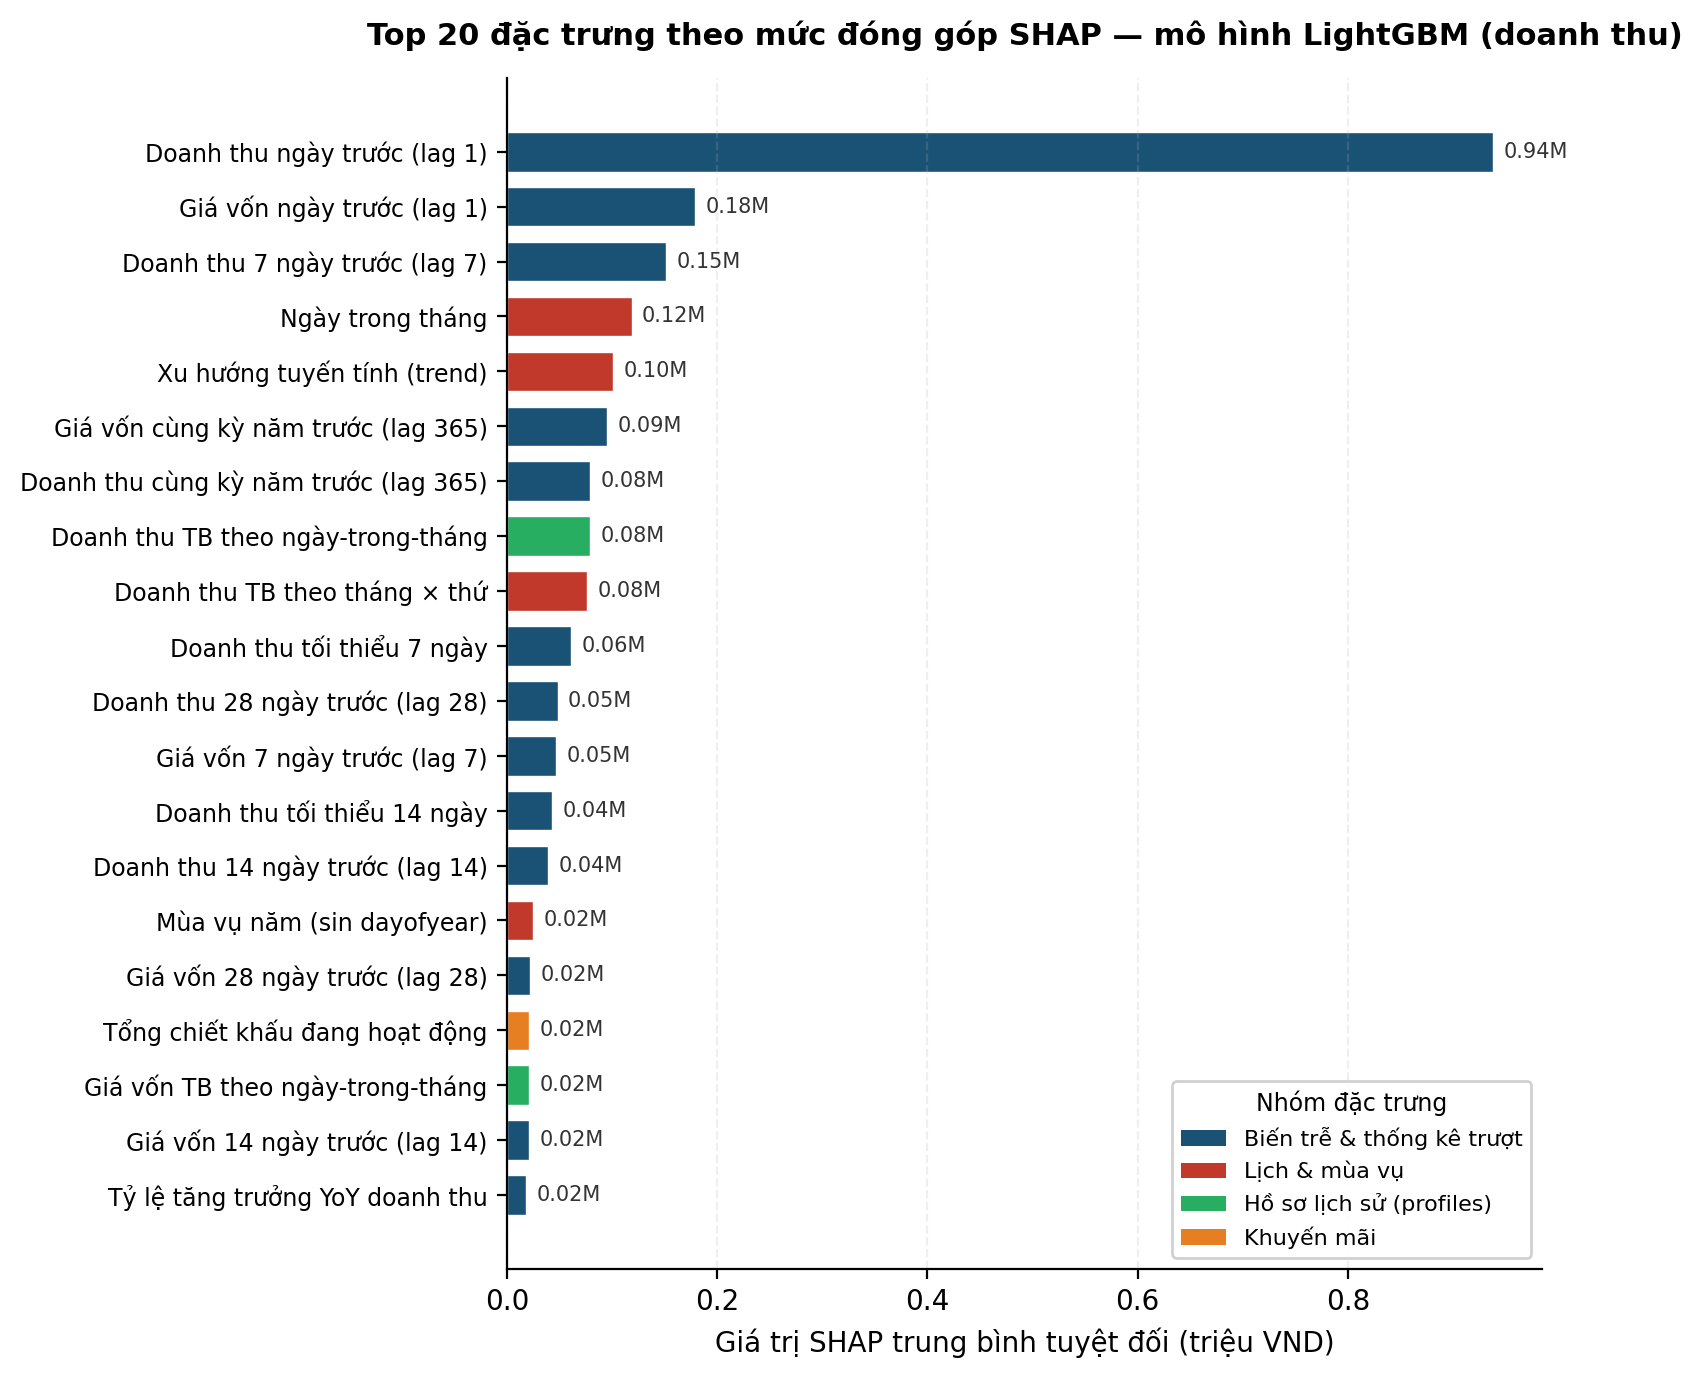
\includegraphics[width=0.82\textwidth]{shap_feature_importance.png}
    \vspace{-0.5em}
    \caption{Top 20 đặc trưng theo giá trị SHAP trung bình tuyệt đối ($\text{mean}\,|\phi_j|$). Màu sắc phân loại: biến trễ \& thống kê trượt (xanh đậm), lịch \& mùa vụ (đỏ), hồ sơ lịch sử (xanh lá), khuyến mãi (cam).}
    \label{fig:shap}
\end{figure}

\begin{figure}[H]
    \centering
    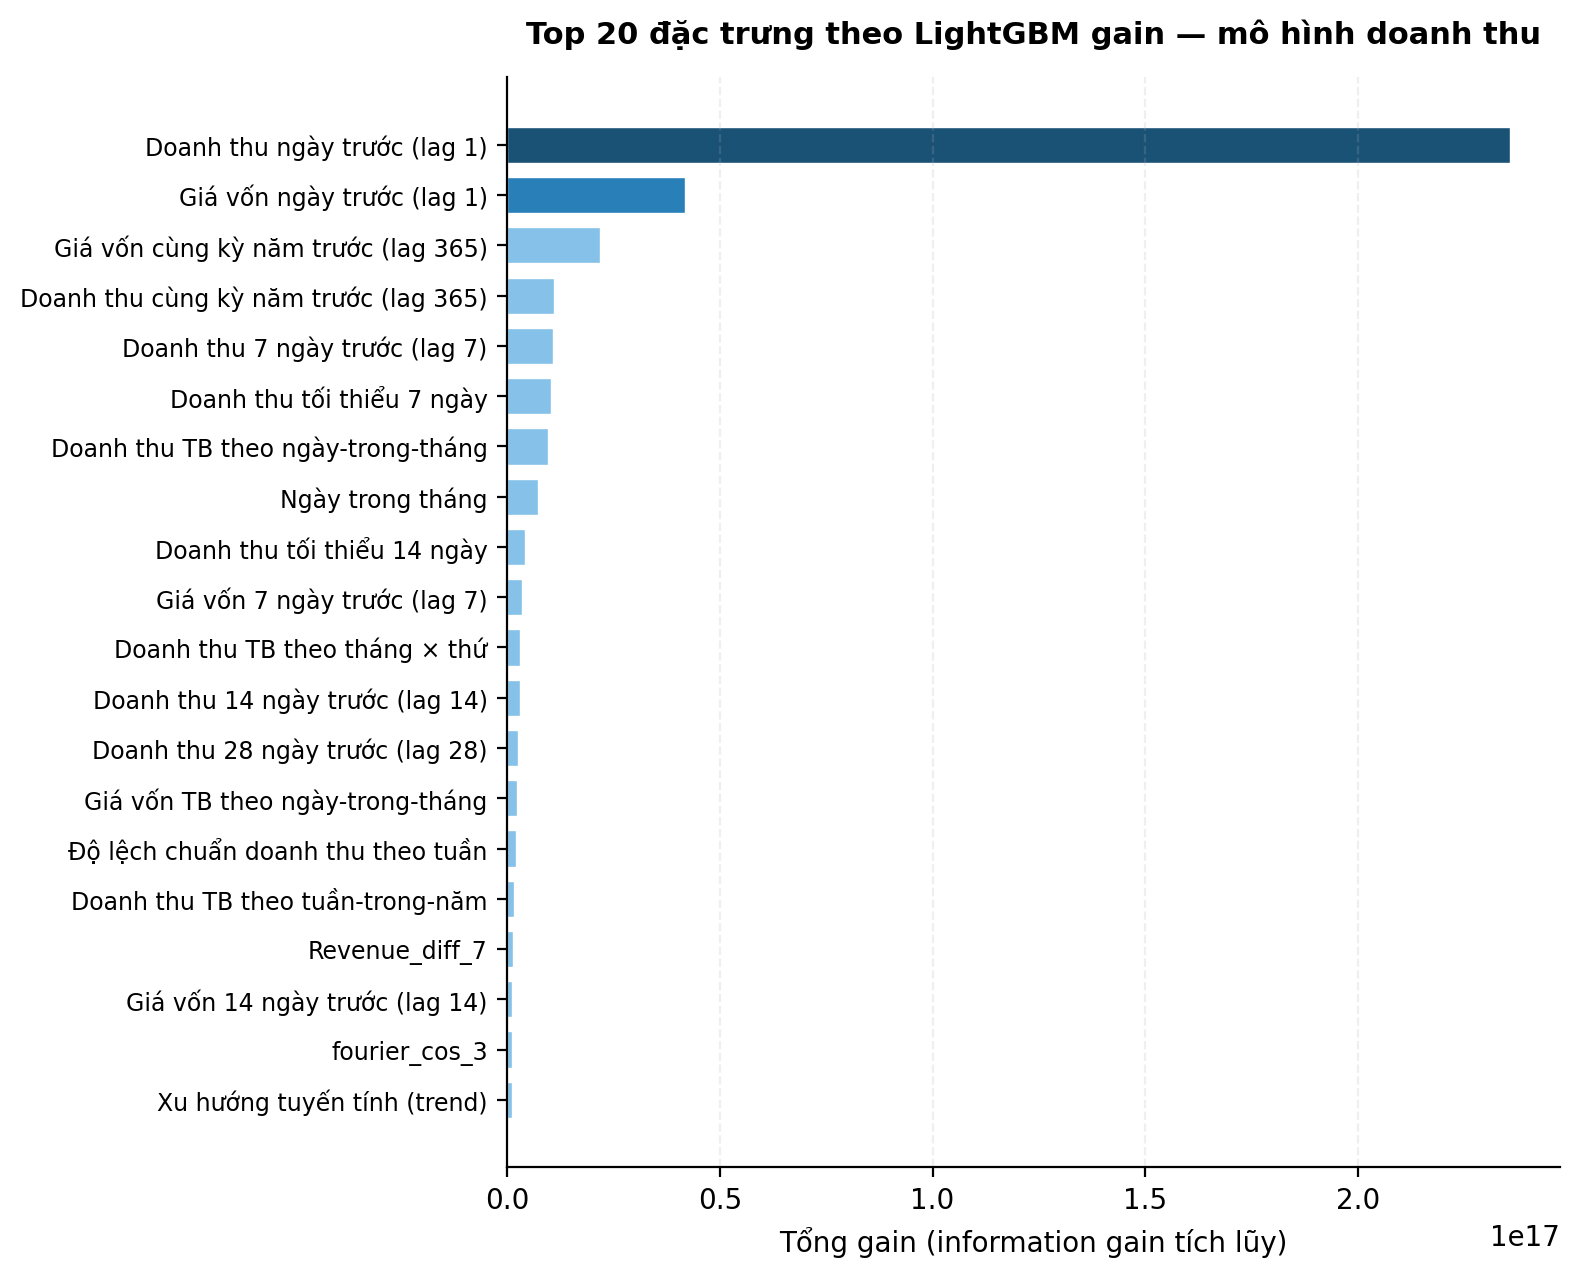
\includegraphics[width=0.78\textwidth]{lgbm_gain_importance.png}
    \vspace{-0.5em}
    \caption{Top 20 đặc trưng theo tổng information gain tích lũy từ cấu trúc cây LightGBM. Cường độ màu tỷ lệ với mức đóng góp tương đối so với đặc trưng hàng đầu.}
    \label{fig:gain}
\end{figure}

\subsubsection{Phân phối tác động theo chiều giá trị đặc trưng:}
Biểu đồ beeswarm (Hình~\ref{fig:beeswarm}) mở rộng phân tích từ giá trị trung bình sang phân phối đầy đủ của các giá trị SHAP. Mỗi điểm biểu diễn một mẫu quan sát, trục hoành thể hiện mức tác động lên dự báo (VND), và màu sắc mã hóa giá trị gốc của đặc trưng (đỏ = cao, xanh = thấp). Một số phát hiện đáng chú ý:
\begin{itemize}[noitemsep,leftmargin=1.2em]
    \item Biến \texttt{Revenue\_lag\_1}: phân phối cho thấy quan hệ đơn điệu dương rõ ràng --- doanh thu hôm trước càng cao thì tác động SHAP càng lớn, xác nhận tính quán tính ngắn hạn.
    \item Biến \texttt{dayofmonth}: giá trị SHAP âm tập trung ở các ngày đầu tháng (xanh) và dương ở cuối tháng (đỏ), phản ánh hiệu ứng chu kỳ lương (payday effect) trong hành vi tiêu dùng.
    \item Biến \texttt{trend}: toàn bộ phân phối nằm trong vùng âm, cho thấy mô hình sử dụng biến xu hướng để điều chỉnh dự báo xuống so với mức cơ sở --- phù hợp với bối cảnh CAGR $-3,80$\%/năm của dữ liệu.
\end{itemize}

\begin{figure}[H]
    \centering
    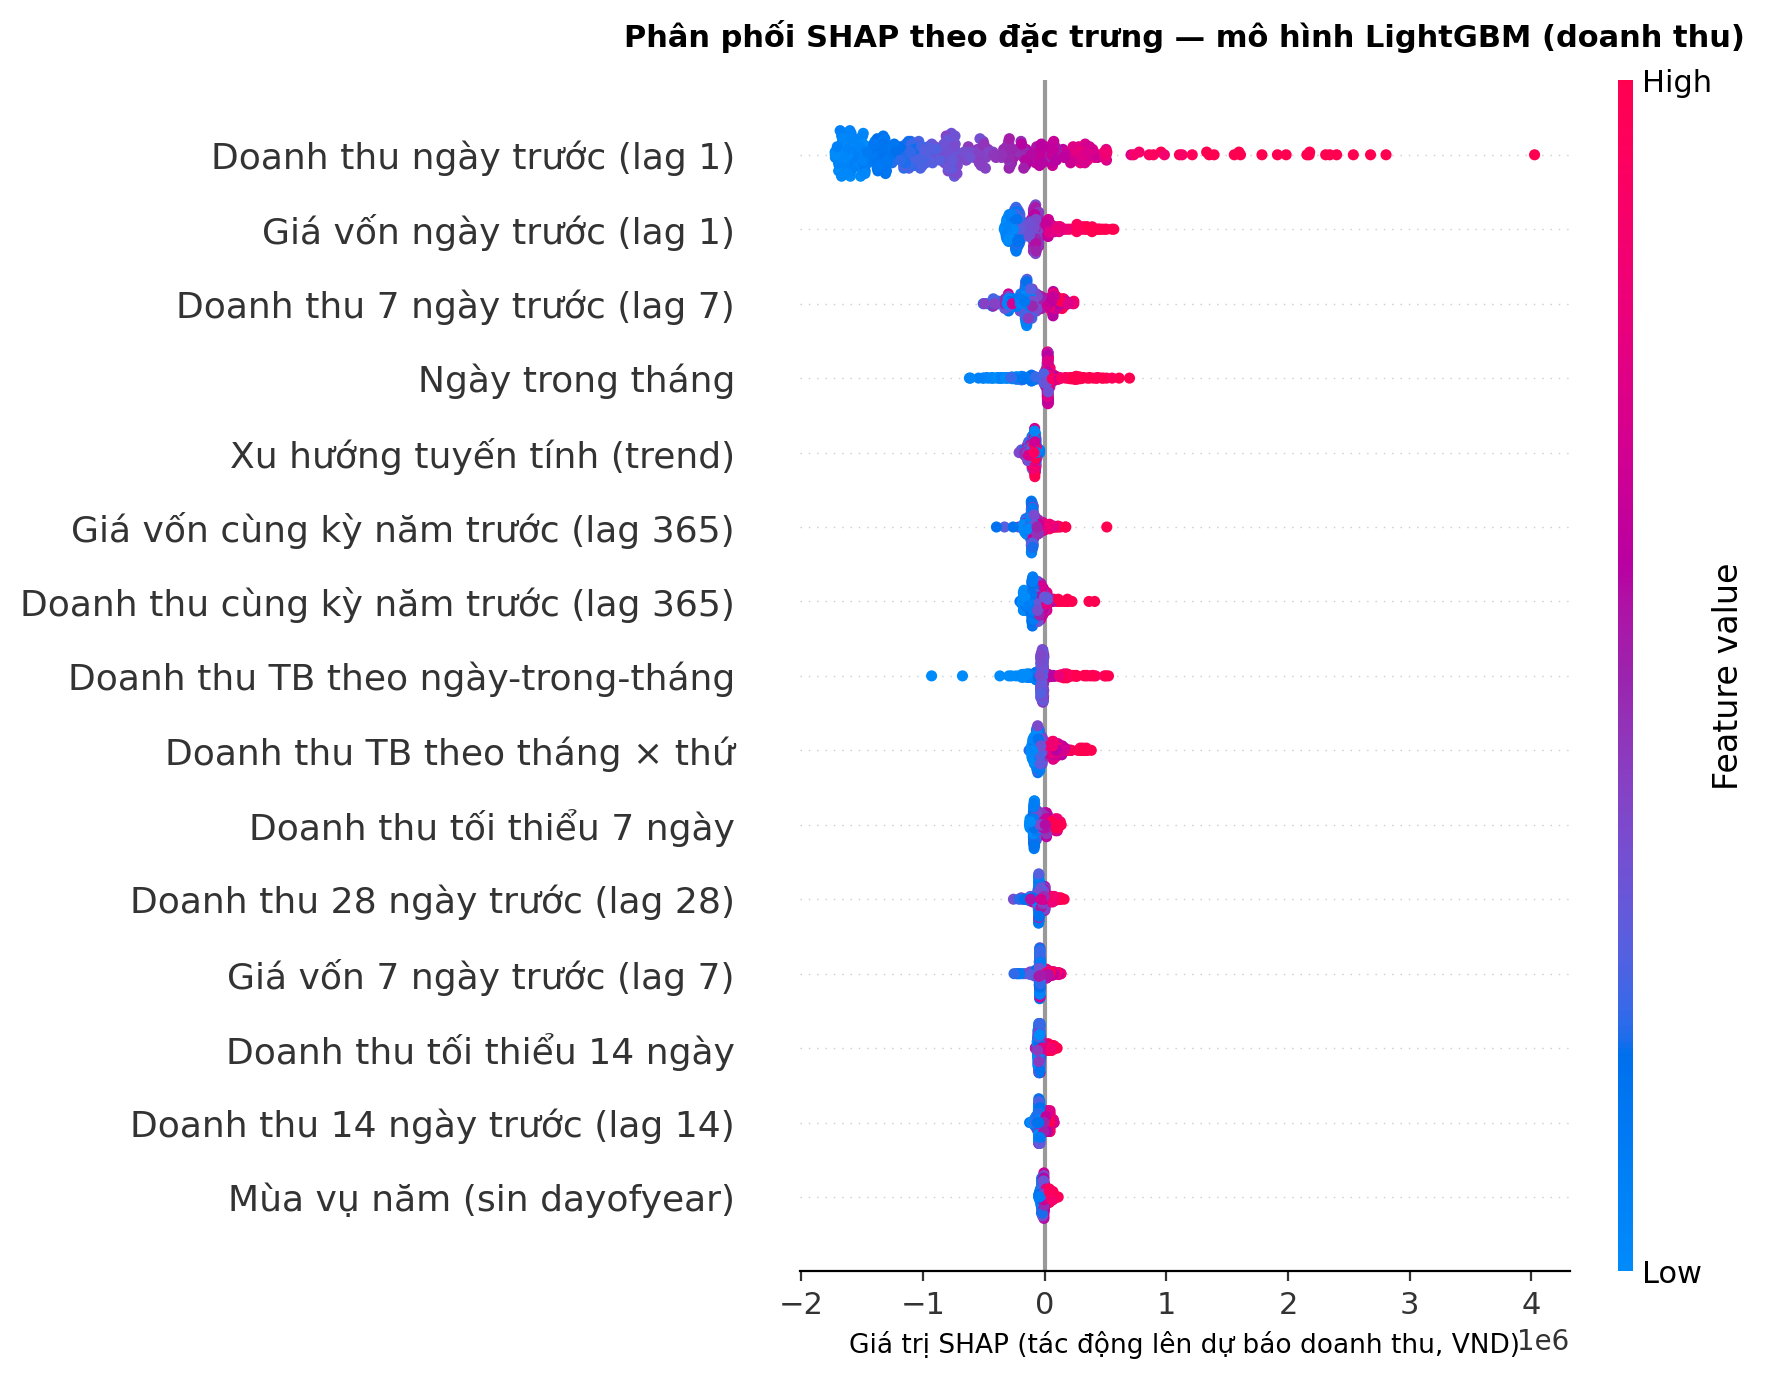
\includegraphics[width=0.82\textwidth]{shap_beeswarm.png}
    \vspace{-0.5em}
    \caption{Biểu đồ beeswarm SHAP cho 15 đặc trưng hàng đầu. Mỗi điểm là một mẫu quan sát; trục hoành là giá trị SHAP (VND); màu sắc mã hóa giá trị gốc của đặc trưng (đỏ = cao, xanh = thấp).}
    \label{fig:beeswarm}
\end{figure}

\subsubsection{Biểu đồ phụ thuộc riêng phần (partial dependence):}
Hình~\ref{fig:dependence} trình bày biểu đồ phụ thuộc SHAP cho bốn đặc trưng có đóng góp cao nhất, giúp làm rõ hàm quan hệ mà mô hình đã học giữa giá trị đặc trưng và tác động lên dự báo:
\begin{itemize}[noitemsep,leftmargin=1.2em]
    \item \texttt{Revenue\_lag\_1}: quan hệ tuyến tính dương với hệ số góc $\approx 0,5$ --- mỗi triệu VND tăng thêm ở doanh thu hôm trước đóng góp khoảng 0,5 triệu VND vào dự báo hôm nay.
    \item \texttt{dayofmonth}: tác động SHAP chuyển từ âm (ngày 1--10) sang dương (ngày 25--31), lượng hóa biên độ hiệu ứng lương cuối tháng ở mức $\pm$400.000--600.000 VND.
    \item \texttt{trend}: tất cả giá trị SHAP đều âm, với biên độ tác động thu hẹp dần theo thời gian, cho thấy mô hình nhận diện xu hướng suy giảm doanh thu dài hạn nhưng với tốc độ giảm dần.
    \item \texttt{Revenue\_lag\_365}: quan hệ dương cho thấy doanh thu cùng kỳ năm trước đóng vai trò mỏ neo (anchor) cho dự báo, với biên độ tác động lên đến +400.000 VND cho các ngày có doanh thu cùng kỳ cao.
\end{itemize}

\begin{figure}[H]
    \centering
    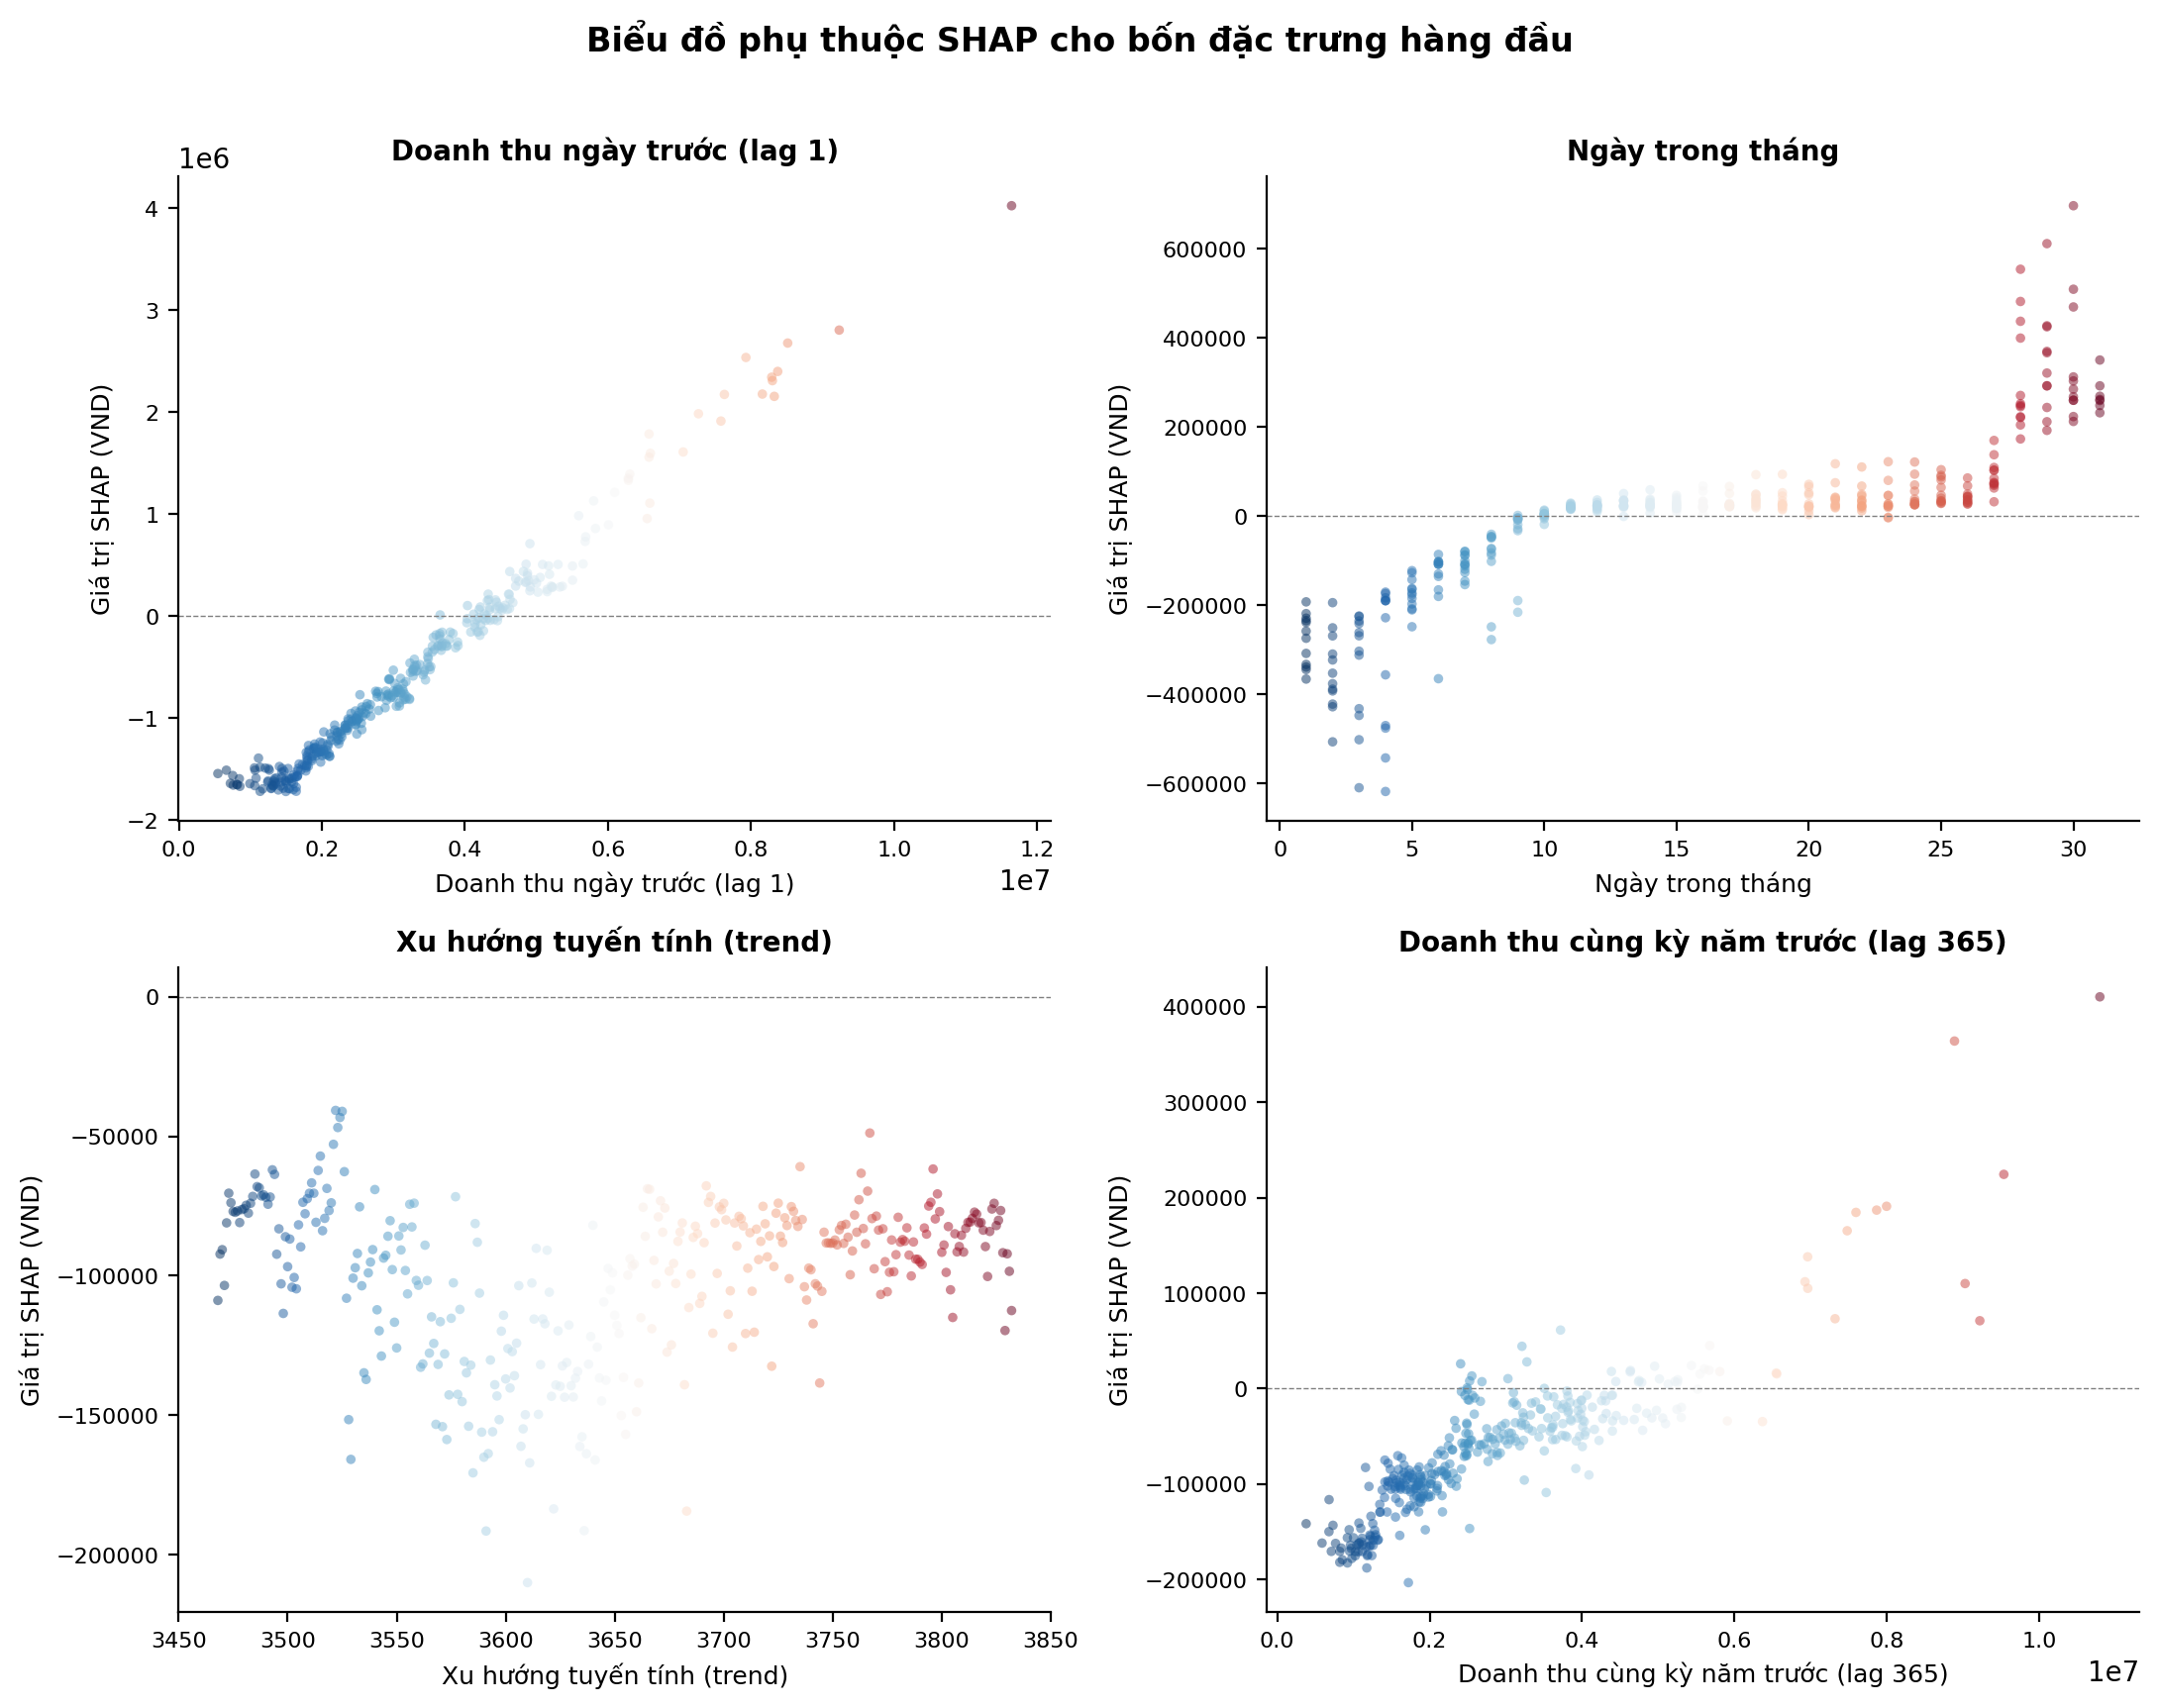
\includegraphics[width=0.7\textwidth]{shap_dependence_top4.png}
    \vspace{-0.5em}
    \caption{Biểu đồ phụ thuộc SHAP cho bốn đặc trưng hàng đầu. Trục hoành: giá trị gốc của đặc trưng; trục tung: giá trị SHAP (VND); màu sắc mã hóa giá trị đặc trưng. Đường nét đứt đánh dấu mức tác động bằng không.}
    \label{fig:dependence}
\end{figure}

Từ góc nhìn kinh doanh, phân tích tổng hợp ba phương pháp trực quan hóa trên xác nhận rằng: (1) doanh thu ngày hôm trước là chỉ báo mạnh nhất, phù hợp với đặc thù bán lẻ thời trang có tính quán tính cao; (2) hiệu ứng lương cuối tháng tạo ra biến động nội tháng có thể lượng hóa; và (3) sự hiện diện của biến \texttt{active\_discount\_sum} cho thấy mô hình đã học được ảnh hưởng trực tiếp của cường độ khuyến mãi lên doanh thu.

\subsection{Tích lũy sai số đệ quy (recursive error accumulation) và giải pháp lai}
Đặc điểm cố hữu làm giới hạn độ chính xác của các mô hình dự báo chuỗi thời gian trong tầm nhìn dài hạn là sự tích lũy sai số đệ quy (recursive error accumulation). 
\begin{itemize}[noitemsep,leftmargin=1.2em]
    \item \textbf{Cơ chế đệ quy (recursive approach):} Phương pháp này ước lượng chính xác mức doanh thu kỳ vọng (base level $\approx$ 3.99 tỷ VND/tháng). Tuy nhiên, sai số ngoại suy cục bộ tại từng bước thời gian lan truyền qua 548 chu kỳ, dẫn đến hiện tượng trôi dạt (drift) xu hướng tuyến tính (ví dụ: dự báo lệch pha từ mức tăng trưởng 5\% trong tháng đầu tiên lên mức định lượng 52\% tại thời điểm tháng thứ 11).
    \item \textbf{Cơ chế phi trạng thái (stateless approach):} Cấu trúc mô hình được tối giản bằng cách loại bỏ các biến đầu vào tự hồi quy, thiết lập hàm quan hệ phụ thuộc hoàn toàn vào đặc trưng thời gian (time-derived features). Cơ chế này loại bỏ triệt để nhiễu đệ quy và duy trì tính ổn định của hàm cấu trúc mùa vụ (seasonality function), nhưng bù lại suy giảm khả năng ước lượng biên độ dao động tổng (chỉ hội tụ ở ngưỡng $\approx$ 3.71 tỷ VND/tháng).
\end{itemize}
\textbf{Giải pháp tích hợp lai (bridge blending):} Để cực đại hóa hiệu quả dự báo, kiến trúc hệ thống áp dụng cơ chế kết hợp (ensemble) có tỷ lệ quy đổi 85\% cho dự báo từ mô hình đệ quy sâu (EX-24) và 15\% từ mô hình phi trạng thái (EX-51). Tại đây, mạng đệ quy đóng vai trò là biến số mỏ neo (anchor) thiết lập trần doanh thu kỳ vọng, trong khi mạng phi trạng thái thực hiện chức năng hiệu chỉnh điều hòa (regularizer), kiểm soát hiện tượng phân kỳ sai số tăng trưởng tại nửa cuối chu kỳ kiểm thử.

\subsection{Tóm tắt thực nghiệm và phân tích cấu trúc mô hình}
Quá trình xây dựng và hiệu chuẩn hệ thống học máy (đạt MAE leaderboard 791,764 từ baseline khởi điểm 1.247M) được thực hiện qua bộ quy trình phân tích với 52 biến thể mô hình. Bảng~\ref{tab:experiments} hệ thống hóa 20 cột mốc nghiên cứu định lượng đóng vai trò định hình lại toàn bộ không gian tham số và phương pháp biểu diễn mô hình. Từ quá trình này, việc quan sát cấu trúc EX-52 đem đến cái nhìn đa chiều về rủi ro của trạng thái lệch pha giữa phân phối tập kiểm định và tập kiểm tra (CV-LB divergence): cơ chế tái hiệu chuẩn (recalibration) chu kỳ tháng dựa trên sai số CV giảm thiểu đáng kể hàm lỗi nội bộ (CV MAE 726k) nhưng gây tổn hại nghiêm trọng lên năng lực nội suy khi đánh giá độc lập (LB MAE 923k).

\begin{table}[H]
\caption{Nhật ký cấu hình các mô hình thực nghiệm cốt lõi (model R\&D tracker)}
\label{tab:experiments}
\centering
\small
\begin{tabular}{@{}llp{7cm}rr@{}}
\toprule
EX & Tên mô hình / cấu trúc & Định nghĩa \& phương pháp cải tiến & CV MAE & LB MAE \\
\midrule
01 & Naive Baseline & Dự báo kỳ vọng qua trung bình mùa vụ quá khứ. & 837,000 & 1,247,026 \\
03 & LightGBM Recursive & Sử dụng tập đặc trưng cơ bản và tự hồi quy. & 560,000 & 973,611 \\
05 & N-HiTS Deep Learning & Kiến trúc mạng nơ-ron dự báo trực tiếp đa bước. & 557,000 & 1,287,946 \\
06 & Weighted Ensemble & Thử nghiệm kết hợp mô hình tuyến tính đơn giản. & - & 861,132 \\
18 & Ensemble-Step Research & Đánh giá hàm lượng thông tin đa mô hình đệ quy. & 570,000 & 859,853 \\
19 & Robust Dual-Weight & Phân phối hàm trọng số hội tụ phi đối xứng. & 599,000 & 834,681 \\
20 & Recency-Weighted & Thiết lập trọng số qua độ tương đồng chu kỳ gần. & 564,000 & 830,584 \\
21 & Deep FE Recency & Bổ sung phân bố cấu trúc hành vi khách hàng mới. & - & 820,000 \\
22 & \textbf{Deep FE Holidays} & \textbf{Tích hợp đặc trưng khoảng cách chu kỳ nghỉ lễ.} & 554,000 & 796,018 \\
24 & \textbf{Deep FE + Double Date} & \textbf{Mô hình đệ quy: tích hợp hiệu ứng sự kiện chuỗi.} & 590,000 & 795,838 \\
25 & Context-Aware FE & Đặc trưng sự kiện nhị phân ngắt quãng (quá khớp). & 617,000 & 842,405 \\
26 & Clean Continuous FE & Lượng hóa nhị phân bằng hàm khoảng cách. & 613,000 & - \\
49 & YoY-Growth Stateless & Cấu trúc phi trạng thái tham chiếu tăng trưởng YoY. & 752,000 & 978,938 \\
50 & Lag-365 Direct Model & Dự báo trực tiếp thông qua biên độ tự hồi quy dài. & 805,000 & - \\
51 & Lag-365 Recursive & Kết hợp Lag-365 và tự hồi quy giữ mức cơ sở. & 769,000 & 917,935 \\
-- & \textit{Bridge Blends (w10)} & Kết hợp lai 90\% đệ quy (EX-24) \& 10\% (EX-51). & - & $\approx$792,300 \\
-- & \textbf{EX-51 Bridge w15} & \textbf{Kiến trúc lai: 85\% đệ quy + 15\% phi trạng thái.} & - & \textbf{791,764} \\
52 & Monthly Recalibration & Tái chuẩn hóa phân phối dư lượng hàng tháng. & \textbf{726,000} & 923,416 \\
52 & Recalib Bridge w15/w30 & Kiểm thử lai có tái hiệu chuẩn dư lượng hàng tháng. & - & $>$798,000 \\
\bottomrule
\end{tabular}
\end{table}

\paragraph{Định hướng mở rộng: mô hình hóa phần dư trực tiếp (residual correction).} 
Nhằm thay thế sự phụ thuộc vào cơ chế hiệu chuẩn hậu kiểm của giải pháp lai (bridge blending), chiến lược lý thuyết tiếp theo tập trung vào cấu trúc học bù trừ (rectify-style). Trong hướng tiếp cận này, sau khi bộ mô hình đệ quy hoàn tất bảo toàn ước lượng doanh thu mức cơ sở (level-preserving), một mạng dự báo trực tiếp (direct models) phân rã theo khối thời gian (như $h \in [1-30]$, $h \in [31-90]$) sẽ được huấn luyện thứ cấp để ước tính véc-tơ phần dư (residuals vector). Điều này kỳ vọng sẽ loại bỏ triệt để hiện tượng sai số lan truyền mà không đòi hỏi thao tác can thiệp thủ công.

% ============================================================
\section{Tổng hợp đề xuất hành động và lộ trình triển khai}
\label{sec:recommendations}

\paragraph{Ma trận tác động $\times$ độ phức tạp.}
Bảng~\ref{tab:actions} tổng hợp sáu đề xuất hành động, sắp xếp theo mức tác động giảm dần. Tổng tác động ước tính đạt \textbf{$\approx$255 triệu VND/năm}, tương đương 21,8\% doanh thu năm 2022 (1,170 tỷ VND).

\begin{table}[H]
\caption{Lộ trình sáu hành động theo tác động, độ phức tạp và thời gian triển khai}
\label{tab:actions}
\centering
\small
\begin{tabular}{@{}clrrll@{}}
\toprule
\# & Hành động & Tác động (tr. VND) & Thời gian & Độ tin cậy & Biểu đồ \\
\midrule
1 & Sàn chiết khấu (floor = COGS$\times$1,15) & \textbf{97} & 2 tuần & Cao & 1.3, 1.4 \\
2 & Thu hút khách hàng miền Trung +30\% & 57 & 3 tháng & Trung bình & 4.1 \\
3 & Kích hoạt RFM (Never Purchased + At Risk) & 38 & 1--2 tháng & Trung bình & 4.2, 4.3 \\
4 & Hướng dẫn size + kiểm định QC Outdoor & 25 & 1 tháng & Cao & 1.2 \\
5 & Nhập hàng 2 lần/tháng --- 10 SKU trọng điểm & 23 & 1--2 tháng & Trung bình & 3.1, 3.2 \\
6 & SLA giao hàng $\leq$ 5 ngày (khi mở rộng) & 15 & 2--3 tháng & Thấp & 5.1 \\
\midrule
& \textbf{Tổng} & \textbf{255} & & & \\
\bottomrule
\end{tabular}
\end{table}

\paragraph{Hệ thống giám sát tự động.}
\textbf{Hàng ngày:} CR $<$ 0,208\% $\Rightarrow$ cảnh báo retargeting. \textbf{Hàng tháng:} bản đồ nhiệt GM\% --- cảnh báo khi $<$12\%; stockout\_days trung bình --- cảnh báo khi $>$1,5 ngày. \textbf{Hàng quý:} tái phân khúc RFM và kiểm tra tỷ lệ giữ chân theo cohort.

\paragraph{Phát hiện phản trực giác cốt lõi.}
Khuyến mãi \textit{không} làm tăng tỷ lệ hoàn trả (lift $\leq 1,00$ trên 714.669 bản ghi). Rủi ro từ khuyến mãi bắt nguồn từ \textit{cấu trúc định giá không phù hợp} khi áp dụng fixed discount lên các phân khúc thiếu biên lợi nhuận đệm (margin buffer). Giải pháp đúng là \textbf{cơ chế kiểm soát sàn giá} (guardrail pricing), không phải cắt giảm khuyến mãi toàn diện.

% ============================================================
\section*{Phụ lục}

\textbf{Tên đội:} The Gridbreakers \quad (4 thành viên).
\textbf{Thành viên:} Nguyễn Ngọc Khoa, Nguyễn Thiên Ấn, Lê Công Minh, Lê Nguyên Khang

\textbf{Mã nguồn:} \url{https://github.com/khoaoe/datathon-2026-gridbreakers}

\textbf{Chú thích biểu đồ:} Toàn bộ 12 biểu đồ (Charts 0.1a, 0.1b, 0.2, 1.1--1.4, 2.1--2.2, 3.1--3.2, 4.1--4.3, 5.1--5.2) bao gồm tiêu đề mô tả, nhãn trục kèm đơn vị, chú giải và ghi chú trên các điểm dữ liệu quan trọng, được tích hợp trong notebook phân tích. Bảng màu thống nhất: Navy Dark (\#001f3f) = doanh thu/chỉ số chính; Vivid Orange = cảnh báo; Red = giá trị âm/tổn thất; Green = giá trị dương.

\end{document}